This section presents the result of testing the Sampling System GUI
in a real case scenario at the ALMA Observatory.
The Sampling System GUI is used in the same deployment as
the operations software (ALMASW).
Figure~\ref{fg:deployment} roughly shows the distributed
environment where ALMASW and the Sampling System GUI are deployed.

\begin{figure}%[b]
  \begin{center}
  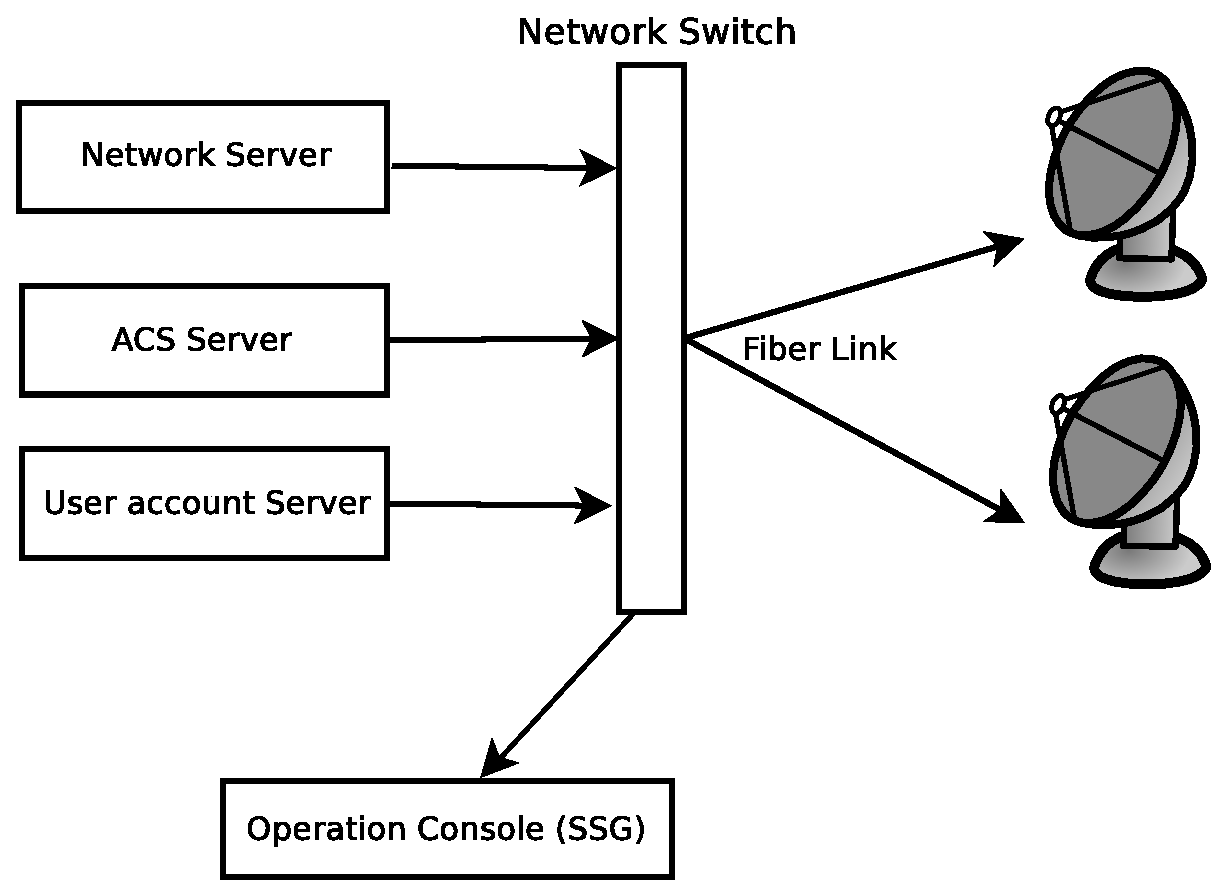
\includegraphics[width=0.50\textwidth]{../img/deployment}
  \end{center}
  \caption{Distributed Deployment}
  \label{fg:deployment}
\end{figure}

ACS and the sampling system run on the ACS server
(figure~\ref{fg:deployment}).
The sampling system GUI is run from the operations console.
This setup was selected to monitor the behavior
of the FrontEnd receiver during its locking routine.
The monitoring setup considered two charts, each with:
\begin{itemize}
\item Five properties being sampled.
\item Sampling frequency of 20\,[Hz].
\item Store a window of 15 minutes of plots.
\item Storing all of the data to disk.
\end{itemize}
20\,[Hz] is the maximum monitoring frequency available in ALMA
since it is limited by its 48\,[ms] period.

The test that was run on the FrontEnd receiver consisted
in locking the band in 0.5\,[GHz] steps over the range of
the four available bands. The test took approximately 4 hours,
time during which the sampling system GUI was
continuously plotting and saving data to disk.
At the time of the test only two antennas were available,
this test should be run again when there are six available antennas
for such purpose. This would demonstrate how the
overall system behaves when increasing the number of distributed
nodes.

The overall result of the Sampling System is positive,
since it met all the engineering requirements for
monitoring during the specified test.
It could cope with the amount of properties and the sampling rates
specified by the engineering division.
Data was properly stored to disk, and the plots
provided a quick look for the data before it was
more thoroughly analyzed.








% real benchmark suite, SSG.


% test cases in a distributed system

%%% Local Variables:
%%% mode: latex
%%% TeX-master: "../article"
%%% End:
